\section*{Zielsetzung}
Bau eines automatischen Coil-Winders für Drahtdurchmesser bis zu AWG 42 (0,0633 mm) klein. Spulenkörper mit kreisförmigen Querschnitt, als auch mit nicht rotationssmetrieschem Querschnitt, sollen sowohl mit paralleler Drahtführung, als auch mit \"wave winding\", oder dem teils randomisierten \"scatter winding\", mehrlagig gewickelt werden können. Für nicht rotationssmetriesche Spulenkörper muss eine automatisches Drahtspannungsvorrichtung konstruiert werden, welche einen zuvor einstellbare Spannung aufrechterhält. Weiters soll die zugehörige Software, bei bekannten Materialparametern und Spulenwiderstand $R$, eigenständig die Wicklungszahl bestimmen.  

\section*{Projektaufbau}

Der Coil-Winder besteht aus einer Hauptachse, auf welcher der Spulenkörper mittels Servo-/Stepper-Motor gedreht wird. Parallel dazu befindet sich eine weitere lineare Achse, auf welcher sich die Drahtführung befindet. Diese wird durch einen Steppermotor, welcher eine Welle dreht, bewegt. Abhängig vom Drahtdurchmesser muss die Führungsspitze natürlich passend gewechselt werden. 

Die Drehzahl des Spulenkörpers muss zur Steuerung bestimmt werden, z.B. mittels eines Hallsensor, oder bei höheren Geschwindigkeiten durch ein optisches System. Des weiteren muss die Position der Drahtführung ständig erfasst werden. Dies könnte durch die Bestimmung einer fixen Startposition, mittels Endschalter, und die Messung der Wellendrehung realisiert werden. Danach kann die Position rechnerisch ermittelt werden. 
\\ 
Um eine gleichmäßige Straffheit der Wicklung zu gewährleisten, muss der aufzuwikelnde Draht stehts eine annähernd konstante Spannung aufweisen. Da es, vorallem bei mehrlagigen Wicklungen, stets zu Beschleunigungsvorgängen der Führungseinheit, und somit zur Erschlaffung des Drahtes, kommt, muss die Spannung mittels einer zusätzlichen Vorrichtung kontinuierlich nachgeregelt werden. Eine Möglichkeit hierfür wäre die konstruktion eines magnetischen Spannsystems, oder einer ähnlichen Vorrichtung.\\
Da eine möglichst hohe Produktionsgeschwindigkeit bei der Wicklung gewünscht ist, muss bei der Planung der Steuereinheit besonderes Augenmerk auf Reaktionsgeschwindigkeit des gesammten Systems gelgegt werden.\\
Auf Softwareseite besteht die Herausforderung hauptsächlich aus der Modellierung des Wicklungsprozesses (vorallem für nicht rotationssmetriesche Spulenkörper), sowie der erstellung des Modells für das Spannsystems und die korrekte Implementation des Regelkreises.\\ 
\\


\begin{figure}[H]
    \centering
    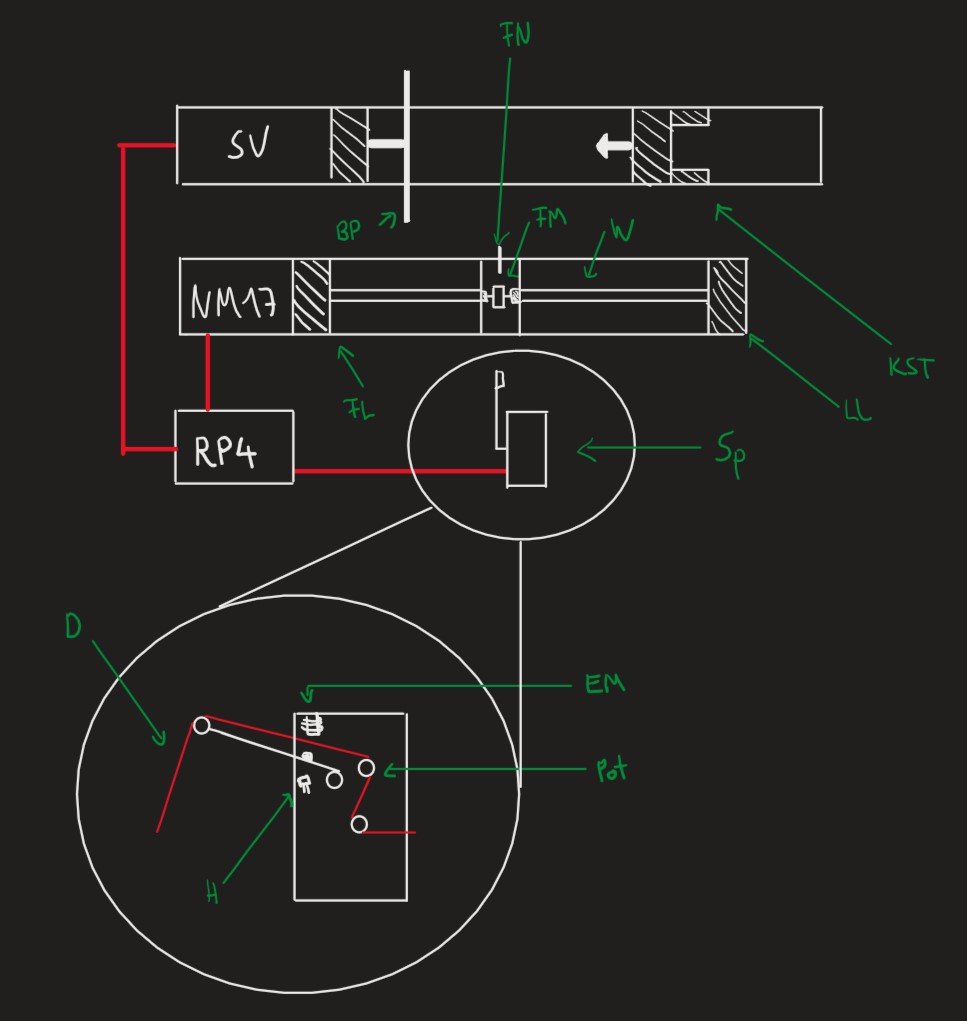
\includegraphics[width=\linewidth]{skizze.jpg}
    \caption{
        Skizze des Spektrographen mit Intensitätsaufnahme optional über Kamera oder Photodiode.
        \textbf{LQ}: Lichtquelle; 
        \textbf{L1,L2,K,F}: Linsen; 
        \textbf{O}: Untersuchungsobjekt; 
        \textbf{S}: Spalt; 
        \textbf{P}: Prismen; 
        \textbf{RP4}: Raspberry Pie 4 zur Datenanalyse; 
        \textbf{Kamera}: direkt an RP4; 
        \textbf{Photodiode}: über ADC an Arduino angeschlossen; 
        \textbf{NEMA 17}: Antrieb für Position der Kamera/Photodiode, über stepper driver an Arduino.
    }
    \label{fig:skizze}
\end{figure}


\section*{Physikalische Anforderungen}
\begin{enumerate}
    \item notwendiger Wellenlängenbereich der Photodiode ca. 300 - 800 nm.
    \item Dimensionen von der Wahl der Linsenbrennweiten abhängig.
    \item Optik muss genug Lichtintensität durchlassen um die Photodiode in einem möglichst linearem Bereich zu betreiben.
    \item Auflösungziel: $\Delta \lambda$ 0,5 nm.
\end{enumerate}


\section*{Komponenten und Kosten}
\begin{table}[H]
    \centering
    \caption{
        Skizze
    }
    \begin{tabular}{| c | c |}
        \hline
        Komponente &  Kosten / \euro{}\\
        \hline
        NEMA 17 (closed loop)& 15 - 60  \\
        \hline
        Stepper Driver & 6 - 10  \\
        \hline
        sonst. Mat. & 50 - 80 \\
        \hline
        Arduino & vorhanden \\
        \hline
        RP4 & vorhanden \\
        \hline
        \hline
        Summe & 110 - 225  \\
        \hline
    \end{tabular}
    \label{tab:Komponenten}
\end{table}



\section*{Software}
\begin{enumerate}
    \item Stepper Steuerung und PhodotiodenIntensitätsmessung ($\mu$C)
    \item Telemetrie, Datenanalyse, Kalibration (RP4 C/C++ und Python)
\end{enumerate}

\section*{Aufwandsabschätzung}
\begin{table}[H]
    \centering
    \caption{
        Skizze
    }
    \begin{tabular}{| c | c |}
        \hline
        Arbeitspaket &  Aufwand / h\\
        \hline
        Optiktisch/Halterungen & 30 - 45  \\
        \hline
        Stepper Steuerung / ADC Messung & 10 - 15 \\
        \hline
        RP4 Telemetrie & 10 - 20  \\
        \hline
        RP4 Datenanalyse & 10 - 20  \\
        \hline
        Kalibration & 20 - 30 \\
        \hline
        Debugging & 50 - 100 \\
        \hline
        \hline
        Summe & 120 - 230  \\
        \hline
    \end{tabular}
    \label{tab:Aufwand}
\end{table}